% *******************************************************************************
% * Copyright (c) 2008 by Elexis
% * All rights reserved. This document and the accompanying materials
% * are made available under the terms of the Eclipse Public License v1.0
% * which accompanies this distribution, and is available at
% * http://www.eclipse.org/legal/epl-v10.html
% *
% * Contributors:
% *    G. Weirich
% *
% *  $Id: anleitung.tex 2417 2007-05-21 04:35:34Z rgw_ch $
% *******************************************************************************

% !Mode:: "TeX:UTF-8" (encoding info for WinEdt)

\documentclass[a4paper]{scrartcl}
\usepackage{german}
\usepackage[utf8]{inputenc}
\usepackage{makeidx}
\makeindex
% Hier ein etwas skurriler Block, der dazu dient, die Unterschiede
% zwischen pdflatex und latex auszubügeln
% Grafiken müssen als png oder gif (für pdflatex) und als eps (für Latex)
% vorhanden sein. Die Endung kann man beim \includegraphics jeweils weglassen,
% das System nimmt je nach Renderer die geeignete Variante.

\usepackage[pdftex]{graphicx}
\DeclareGraphicsExtensions{.pdf,.jpg,.png}

\usepackage{floatflt}
\usepackage[]{hyperref}
\usepackage{color}

\begin{document}
\title{Basis-Buchhaltungsfunktionen für Elexis}
\author{Gerry Weirich}
\maketitle

\section{Einführung}
Dieses Plugin bietet einige grundlegende Buchhaltungsfunktionen wie FakturaJournal, Zahlungsjournal und Debitoren per Datum.

\subsection{Voraussetzungen}
Elexis-buchhaltung-basis benötigt Elexis 1.4 oder höher. Ausserdem muss das Plugin 'Archie' (http://archie.designchuchi.ch) installiert sein. Buchhaltung-Basis hängt sich in die Archie-Statistikauswahl ein.

\subsection{Installation und Deinstallation}
Wie üblich muss das Plugin zur Installation nur in den Plugins-Ordner kopiert bzw. zur Deinstallation aus diesem Ordner gelöscht werden. Danach muss Elexis neu gestartet werden.

\section{Bedienung}
Gehen Sie für alle im Weiteren beschriebenen Auswertungen auf die Archie-Perspektive (S. Abb. \ref{fig:buch1}). Die gewünschte Auswertung kann in der Combobox rechts oben ('Verfügbare Statistiken') ausgesucht werden, im Feld darunter können Parameter wie Start- und Enddatum eingestellt werden, und schliesslich wird die Analyse durch Klick auf 'Abfrage starten' ausgelöst. Das Ergebnis erscheint dann im linken Fenster und kann - wie alle in Archie erstellten Auswertungen - grafisch angezeigt oder im universellen CSV-Format für andere Programme wie Excel\texttrademark exportiert werden.

\medskip

Aus Datenschutzgründen werden keine Patientennamen sondern nur die internen -- und für Dritte bedeutungslosen -- Patientennummern angegeben. Die Liste kann daher ohne Bedenken z.B. einem Treuhänder oder WIrtschatsprüfer übergeben werden.


\begin{figure}
  % Requires \usepackage{graphicx}
  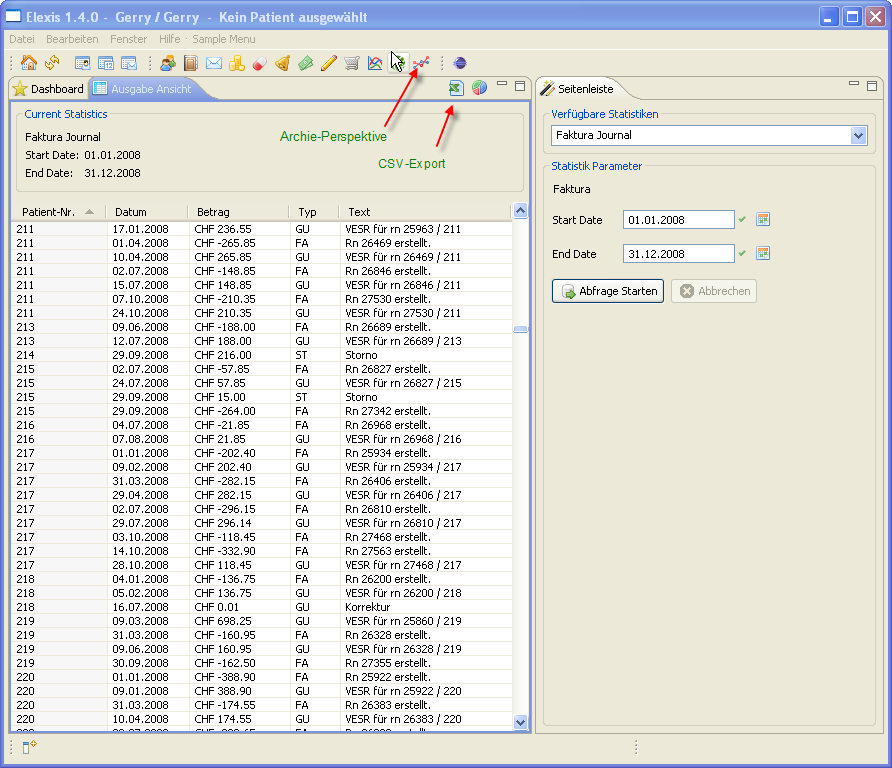
\includegraphics[width=0.9\textwidth]{buch1}\\
  \caption{Elexis-Buchhaltung in Archie}\label{fig:buch1}
\end{figure}

\subsection{Faktura-Journal}
Diese Auswertung liefert Ihnen alle im angegebenen Zeitraum ausgelösten Buchungsvorgänge (Rechnungen, Zahlungen, Stornos). Der Saldo aller Buchungsvorgänge entspricht Ihren offenen Debitoren.

Wählen Sie dazu unter 'Verfügbare Statistiken' die Option 'Faktura-Journal', wählen Sie Start- und Enddatum und klicken Sie auf 'Abfrage starten';

\subsection{Zahlungsjournal}
Diese Auswertung liefert alle Zahlungseingänge im angegebenen Zeitraum.

\subsection{Offene Posten}

\begin{figure}[htbp]
    \begin{minipage}{0.5\textwidth}
      \centering
       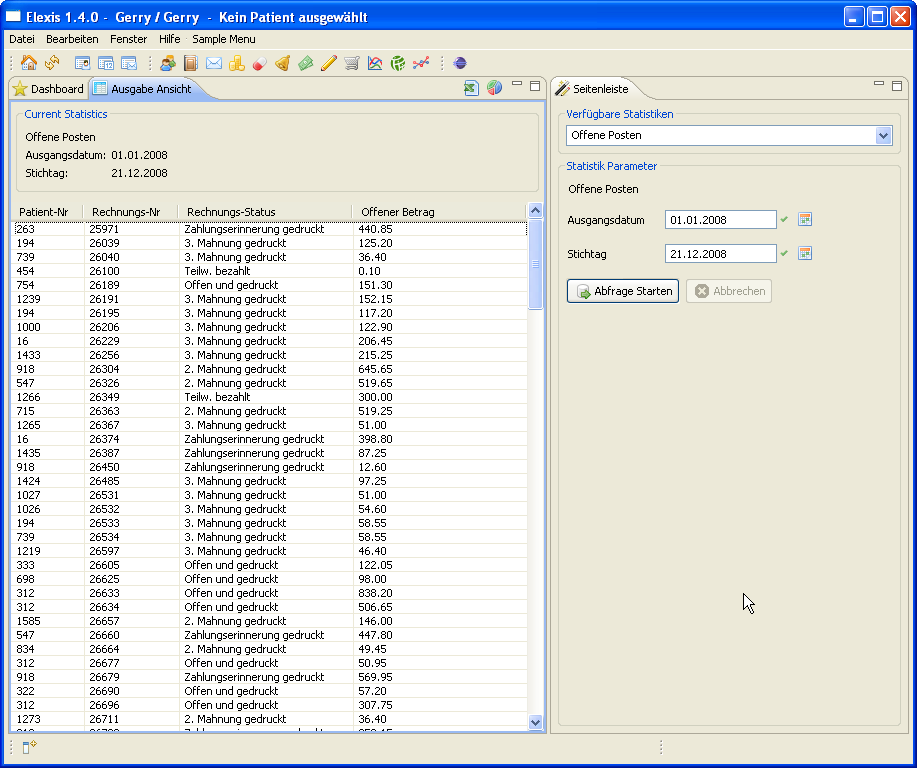
\includegraphics[width=0.95\textwidth]{buch2}
         \caption{Offene Posten Auswertung}\label{fig:buch2}
     \end{minipage}\hfill
     \begin{minipage}{0.5\textwidth}
      \centering
       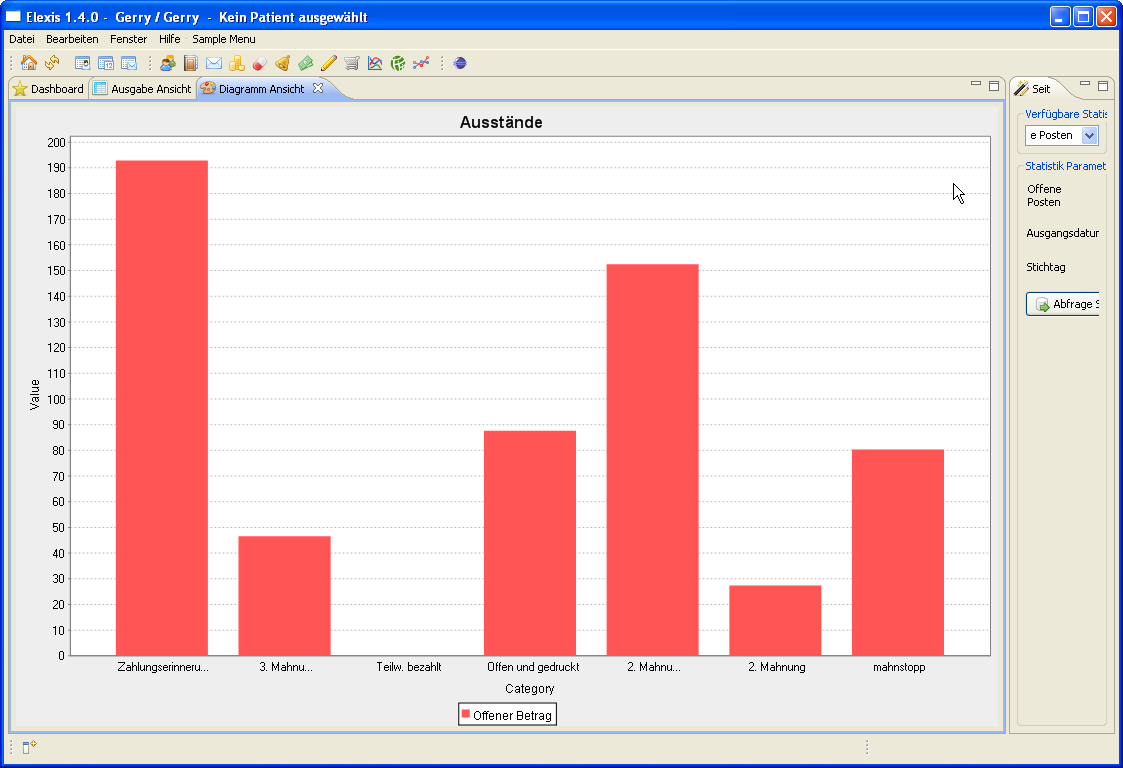
\includegraphics[width=0.95\textwidth]{buch3}
       \caption{Offene Posten grafisch}\label{fig:buch3}
    \end{minipage}
\end{figure}


Diese Auswertung (Vgl. Abb. \ref{fig:buch2})liefert alle Ausstände zu einem anzugebenden Stichtag. Wählen Sie das Ausgangsdatum (ältere Rechnungen werden nicht mehr berücksichtigt) und einen Stichtag (Zahlungen nach diesem Stichtag werden nicht mehr berücksichtigt). Abb. \ref{fig:buch3} zeigt ein Beispiel, wie man eine Auswertung grafisch darstellen kann, hier Betrags-Vergleich der verschiedenen Kategorien von Ausständen.

\subsection{Rechnungen nach Fälligkeitsdatum}
Diese Auswertung erlaubt Ihnen eine gewissen 'Blick in die Zukunft': Sie zeigt Ihnen, welche Rechnungen bis zu einem bestimmten Zeitpunkt fällig werden.
Geben Sie das gewünschte Stichdatum ein und klicken Sie auf 'Abfrage starten'.

\end{document} 